\documentclass[aspectratio=169,10pt]{beamer}

\usetheme{Madrid}
\usecolortheme{default}
\setbeamertemplate{navigation symbols}{}
\setbeamertemplate{footline}[frame number]
\setbeamertemplate{itemize items}[circle]
\setbeamertemplate{enumerate items}[default]

\usepackage[T1]{fontenc}
\usepackage[utf8]{inputenc}
\usepackage{lmodern}
\usepackage{booktabs}
\usepackage{graphicx}
\usepackage{array}
\usepackage{xcolor}
\usepackage{amsmath}

\definecolor{ColumbiaBlue}{RGB}{0,114,178}
\definecolor{DarkGray}{RGB}{45,45,45}
\definecolor{LightGray}{RGB}{245,247,250}
\setbeamercolor{structure}{fg=ColumbiaBlue}
\setbeamercolor{frametitle}{fg=DarkGray,bg=LightGray}
\setbeamercolor{title}{fg=DarkGray}
\setbeamercolor{block title}{fg=white,bg=ColumbiaBlue}
\setbeamercolor{block body}{bg=LightGray}

\title[Multi-Agent Protocol Study]{Communication Protocol Effects on Multi-Agent System Efficiency and Task Completion}
\subtitle{STAT GR5293 Final Project Presentation}
\author{Yi Zhang \and Xian Zhang \and Tianyu Zhan}
\institute{Department of Statistics, Columbia University}
\date{Spring 2026}

\newcommand{\protocol}[1]{\texttt{#1}}
\newcommand{\metric}[1]{\textbf{#1}}

\begin{document}

\begin{frame}
  \titlepage
\end{frame}

\begin{frame}{Presentation Roadmap}
  \begin{columns}[T,onlytextwidth]
    \begin{column}{0.32\textwidth}
      \begin{block}{Problem Statement}
        Why communication format is an uncontrolled design choice in multi-agent LLM systems.
      \end{block}
    \end{column}
    \begin{column}{0.32\textwidth}
      \begin{block}{Major Contributions}
        Controlled protocol comparison, reusable pipeline, statistical analysis, and a live demo.
      \end{block}
    \end{column}
    \begin{column}{0.32\textwidth}
      \begin{block}{Evaluation}
        360 pipeline runs across four protocols, three domains, and multiple efficiency and quality metrics.
      \end{block}
    \end{column}
  \end{columns}

  \vspace{0.45cm}
  \textbf{Rubric alignment:} the presentation is organized around the three 10\% final-presentation categories: problem statement, contributions, and evaluation.
\end{frame}

\begin{frame}{Problem Statement}
  Multi-agent LLM systems are increasingly built as pipelines: agents plan, execute, critique, retrieve, or integrate intermediate work.

  \vspace{0.25cm}
  Most frameworks expose inter-agent communication as a flexible engineering choice, but do not answer a basic empirical question:

  \begin{block}{Core Question}
    How does the communication protocol between agents change token cost, latency, and task completion quality?
  \end{block}

  \begin{itemize}
    \item The protocol can be plain natural language, Markdown, JSON, or a shared blackboard.
    \item The same protocol may not be optimal for math, reading comprehension, and news analysis.
    \item The practical target audience is developers choosing protocols in LangGraph, AutoGen, CrewAI, or custom agent systems.
  \end{itemize}
\end{frame}

\begin{frame}{Research Questions and Hypotheses}
  \begin{table}
    \centering
    \small
    \begin{tabular}{p{0.18\textwidth}p{0.42\textwidth}p{0.30\textwidth}}
      \toprule
      & Question & Hypothesis \\
      \midrule
      RQ1 & How much does protocol choice affect efficiency? & Shared memory costs the most tokens; structured formats should reduce ambiguity. \\
      RQ2 & How much does protocol choice affect task completion? & Protocol effects may vary by domain and evaluator. \\
      RQ3 & Is there a protocol-by-domain interaction? & The best protocol should change across math, reading, and news. \\
      \bottomrule
    \end{tabular}
  \end{table}

  \vspace{0.15cm}
  \textbf{Scope boundary:} the project studies the protocol layer, not a new task-specific agent application.
\end{frame}

\begin{frame}{System Model}
  \begin{columns}[T,onlytextwidth]
    \begin{column}{0.48\textwidth}
      \textbf{Fixed three-agent chain}
      \begin{enumerate}
        \item Planning Agent: decomposes the task.
        \item Execution Agent: completes subtasks.
        \item Integration Agent: produces the final answer.
      \end{enumerate}

      \vspace{0.2cm}
      Held constant across all conditions:
      \begin{itemize}
        \item model: \protocol{gpt-4o-mini}
        \item temperature: 0.3
        \item agent roles and system prompts
        \item max tokens by domain
      \end{itemize}
    \end{column}
    \begin{column}{0.48\textwidth}
      \textbf{Manipulated factor: protocol}
      \begin{itemize}
        \item \protocol{NL}: explicit plain-prose instruction.
        \item \protocol{MARKDOWN}: headings and bullet structure.
        \item \protocol{JSON}: valid JSON object with parse validation and one retry.
        \item \protocol{SHARED\_MEMORY}: global blackboard; every agent reads the full state snapshot.
      \end{itemize}

      \vspace{0.2cm}
      \begin{block}{Design Principle}
        Change the message format, not the agent architecture.
      \end{block}
    \end{column}
  \end{columns}
\end{frame}

\begin{frame}{Experimental Design}
  \begin{columns}[T,onlytextwidth]
    \begin{column}{0.48\textwidth}
      \textbf{Factorial grid}
      \begin{itemize}
        \item 4 protocols: \protocol{NL}, \protocol{MARKDOWN}, \protocol{JSON}, \protocol{SHARED\_MEMORY}
        \item 3 domains: GSM8K math, SQuAD reading, curated news
        \item 10 samples per domain
        \item 3 repetitions per cell
      \end{itemize}

      \vspace{0.2cm}
      \[
        4 \times 3 \times 10 \times 3 = 360 \text{ pipeline runs}
      \]
    \end{column}
    \begin{column}{0.48\textwidth}
      \textbf{Metrics}
      \begin{itemize}
        \item Efficiency: prompt tokens, completion tokens, total tokens.
        \item Runtime: wall-clock latency.
        \item Quality:
          numeric exact match for math,
          SQuAD token-F1 for reading,
          mean ROUGE-2/ROUGE-L F1 for news.
      \end{itemize}

      \vspace{0.2cm}
      \textbf{Inference}
      \begin{itemize}
        \item Two-way ANOVA, Tukey HSD, Cohen's $d$.
        \item 2,000-resample bootstrap confidence intervals.
      \end{itemize}
    \end{column}
  \end{columns}
\end{frame}

\begin{frame}{Contribution 1: Controlled Protocol Benchmark}
  \begin{itemize}
    \item A reusable experiment harness separates the protocol factor from agent roles and task data.
    \item Every inter-agent message is logged with sender, receiver, content, token split, latency, finish reason, and parse-error status.
    \item The resulting dataset contains 360 run summaries and 1,080 message records.
  \end{itemize}

  \vspace{0.25cm}
  \begin{table}
    \centering
    \small
    \begin{tabular}{lccc}
      \toprule
      Artifact & File & Purpose & Rubric Value \\
      \midrule
      Pipeline & \protocol{pipeline.py} & reproducible experiment runner & technical depth \\
      Results & \protocol{results/*.csv/jsonl} & quantitative evidence & evaluation \\
      Figures & \protocol{figures/*.png} & presentation/report visuals & clarity \\
      Demo & \protocol{app.py} & end-to-end protocol selector & practical impact \\
      \bottomrule
    \end{tabular}
  \end{table}
\end{frame}

\begin{frame}{Result: Protocol Strongly Affects Token Cost}
  \begin{columns}[T,onlytextwidth]
    \begin{column}{0.58\textwidth}
      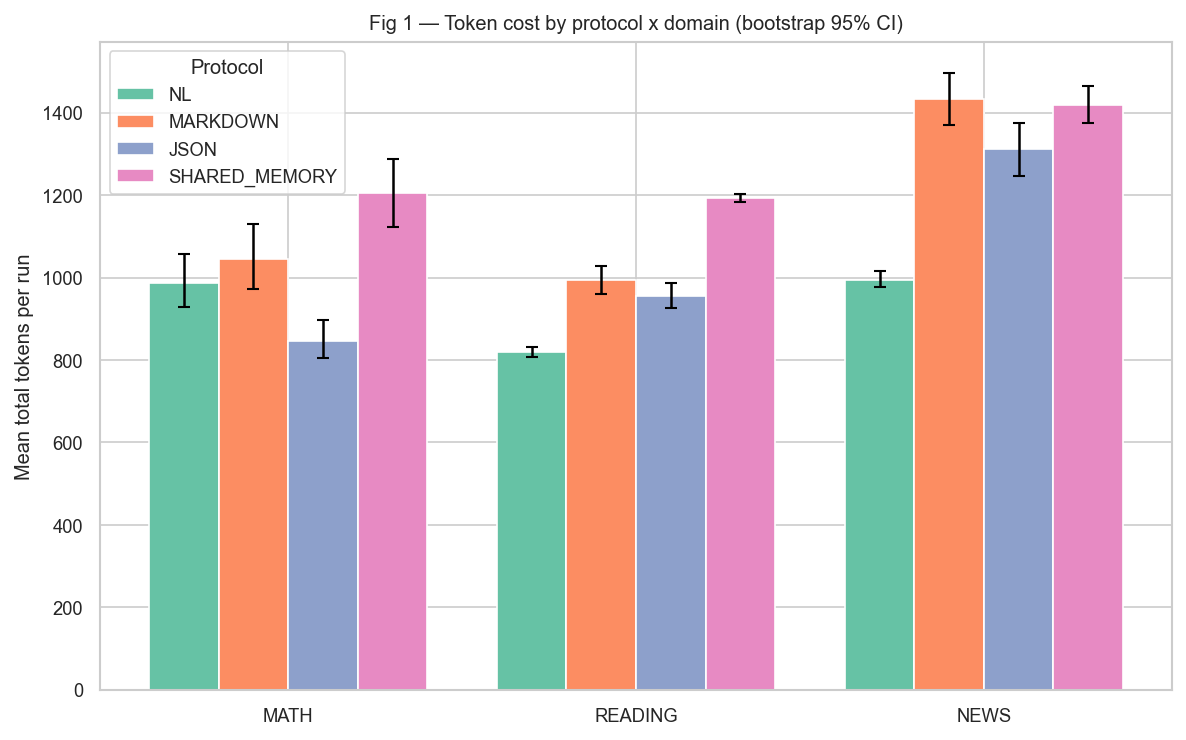
\includegraphics[width=\textwidth]{../figures/fig1_tokens_by_protocol_domain.png}
    \end{column}
    \begin{column}{0.39\textwidth}
      \textbf{Two-way ANOVA on total tokens}
      \begin{table}
        \centering
        \tiny
        \begin{tabular}{lccc}
          \toprule
          Term & F & p & $\eta^2$ \\
          \midrule
          Protocol & 87.40 & $<.001$ & .262 \\
          Domain & 148.19 & $<.001$ & .296 \\
          Protocol $\times$ domain & 15.66 & $<.001$ & .094 \\
          \bottomrule
        \end{tabular}
      \end{table}

      \vspace{0.1cm}
      \textbf{Verdict:} Shared memory is the most expensive protocol in every domain, averaging +338 tokens per run versus \protocol{NL}.
    \end{column}
  \end{columns}
\end{frame}

\begin{frame}{Why the Cost Changes}
  \begin{columns}[T,onlytextwidth]
    \begin{column}{0.58\textwidth}
      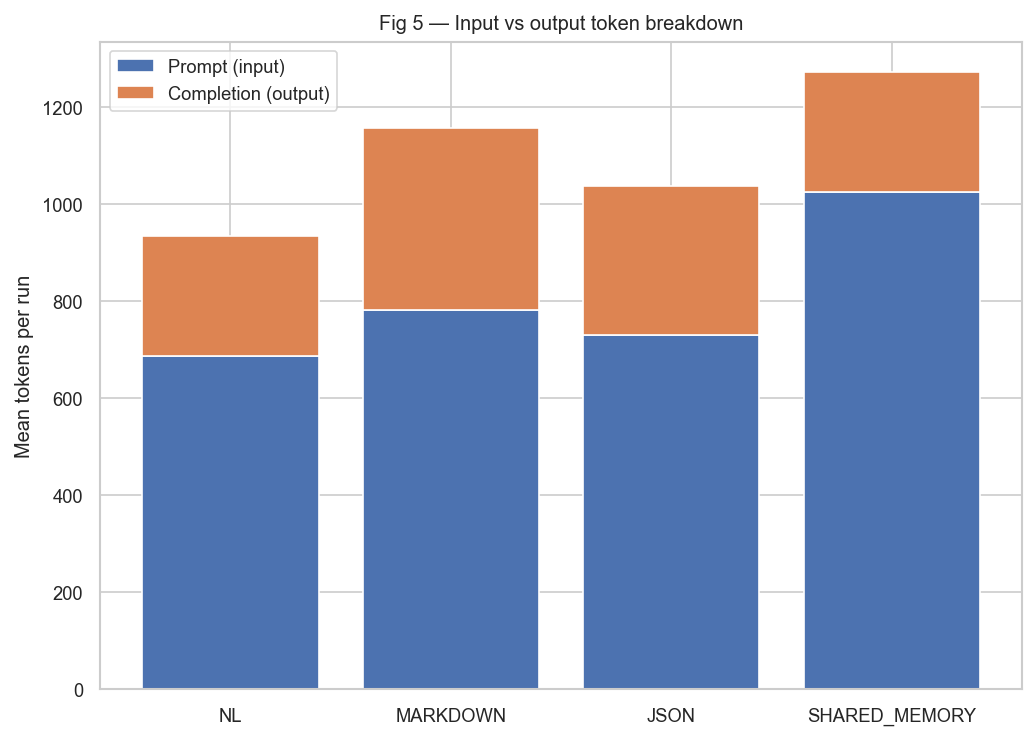
\includegraphics[width=\textwidth]{../figures/fig5_input_vs_output.png}
    \end{column}
    \begin{column}{0.39\textwidth}
      \begin{itemize}
        \item \protocol{SHARED\_MEMORY} inflates prompt tokens because downstream agents receive the full blackboard snapshot.
        \item \protocol{MARKDOWN} often increases completion tokens because headings and bullets add verbosity.
        \item \protocol{JSON} is cheapest on math, but not pooled-cheapest overall.
        \item \protocol{NL} is a strong budget default for reading and news.
      \end{itemize}

      \vspace{0.2cm}
      \begin{block}{Efficiency Ordering}
        Pooled token cost: \protocol{NL} $<$ \protocol{JSON} $<$ \protocol{MARKDOWN} $<$ \protocol{SHARED\_MEMORY}
      \end{block}
    \end{column}
  \end{columns}
\end{frame}

\begin{frame}{Result: Quality Effects Are Domain-Dependent}
  \begin{columns}[T,onlytextwidth]
    \begin{column}{0.58\textwidth}
      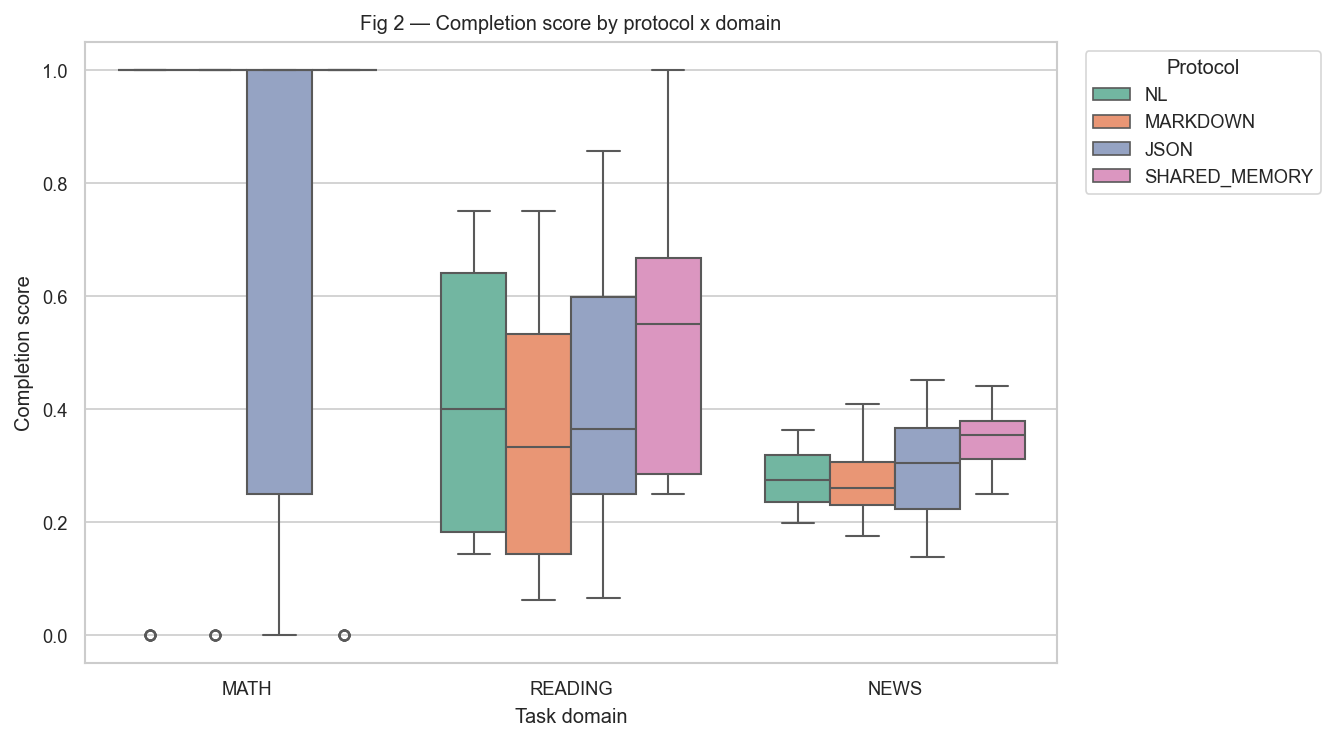
\includegraphics[width=\textwidth]{../figures/fig2_completion_by_cell.png}
    \end{column}
    \begin{column}{0.39\textwidth}
      \textbf{Per-domain ANOVA on completion}
      \begin{table}
        \centering
        \tiny
        \begin{tabular}{lcccc}
          \toprule
          Domain & F & p & $\eta^2$ & Best \\
          \midrule
          Math & 0.66 & .58 & .017 & Markdown \\
          Reading & 4.39 & .006 & .102 & Shared mem. \\
          News & 9.51 & $<.001$ & .197 & Shared mem. \\
          \bottomrule
        \end{tabular}
      \end{table}

      \vspace{0.1cm}
      \textbf{Verdict:} protocol choice is mostly a cost lever for math, but a quality lever for reading and news.
    \end{column}
  \end{columns}
\end{frame}

\begin{frame}{Interaction Pattern}
  \begin{columns}[T,onlytextwidth]
    \begin{column}{0.58\textwidth}
      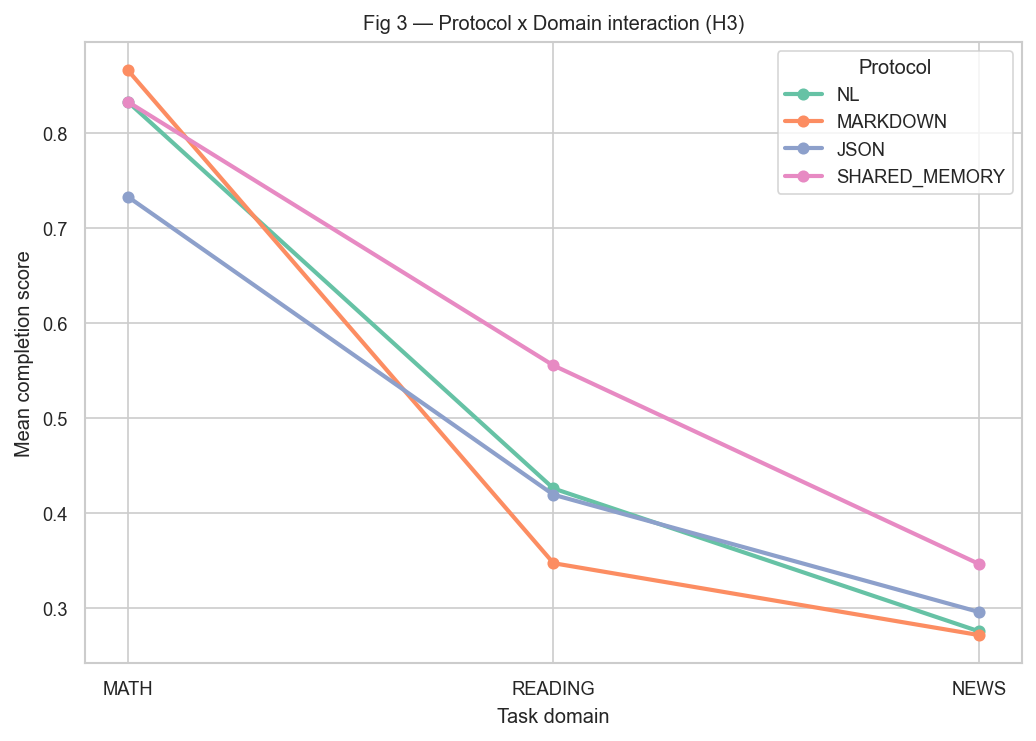
\includegraphics[width=0.94\textwidth]{../figures/fig3_interaction.png}
    \end{column}
    \begin{column}{0.39\textwidth}
      \small
      \begin{itemize}
        \item The best protocol changes by domain.
        \item Math: protocols cluster closely; Markdown leads by a small margin.
        \item Reading: shared memory preserves passage context and improves token-F1.
        \item News: shared memory preserves facts and figures better.
      \end{itemize}

      \vspace{0.08cm}
      \begin{block}{Statistical Note}
        Pooled completion interaction: $p=.203$; per-domain effect sizes range from .017 to .197.
      \end{block}
    \end{column}
  \end{columns}
\end{frame}

\begin{frame}{Efficiency--Effectiveness Trade-off}
  \begin{columns}[T,onlytextwidth]
    \begin{column}{0.58\textwidth}
      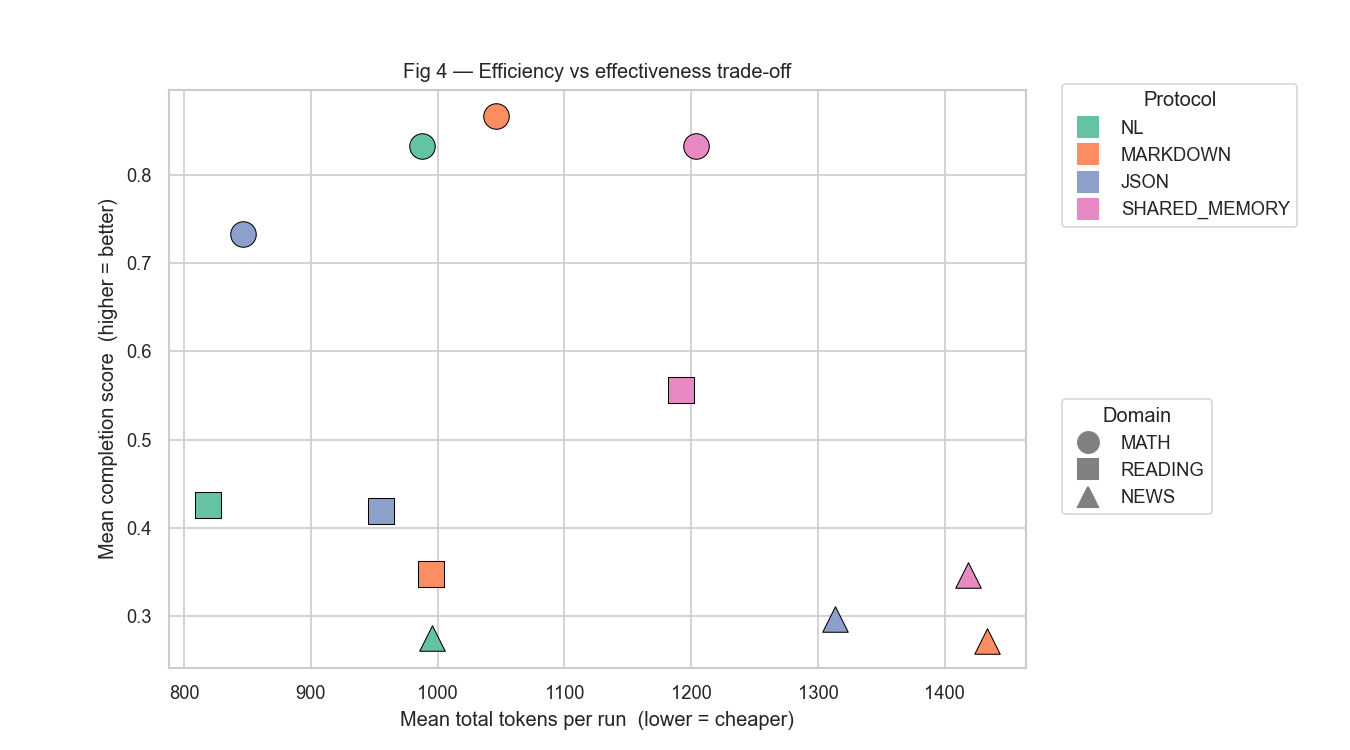
\includegraphics[width=\textwidth]{../figures/fig4_pareto.png}
    \end{column}
    \begin{column}{0.39\textwidth}
      \textbf{Practitioner recommendation}
      \begin{itemize}
        \item Math: choose \protocol{MARKDOWN} for best completion, \protocol{JSON} for lowest cost.
        \item Reading: choose \protocol{SHARED\_MEMORY} for quality; \protocol{NL} for budget.
        \item News: choose \protocol{SHARED\_MEMORY} when factual completeness matters.
      \end{itemize}

      \vspace{0.2cm}
      \begin{block}{Main Trade-off}
        Shared memory buys quality on open-text tasks, but it is never the cheapest option.
      \end{block}
    \end{column}
  \end{columns}
\end{frame}

\begin{frame}{Latency and Operational Cost}
  \begin{columns}[T,onlytextwidth]
    \begin{column}{0.58\textwidth}
      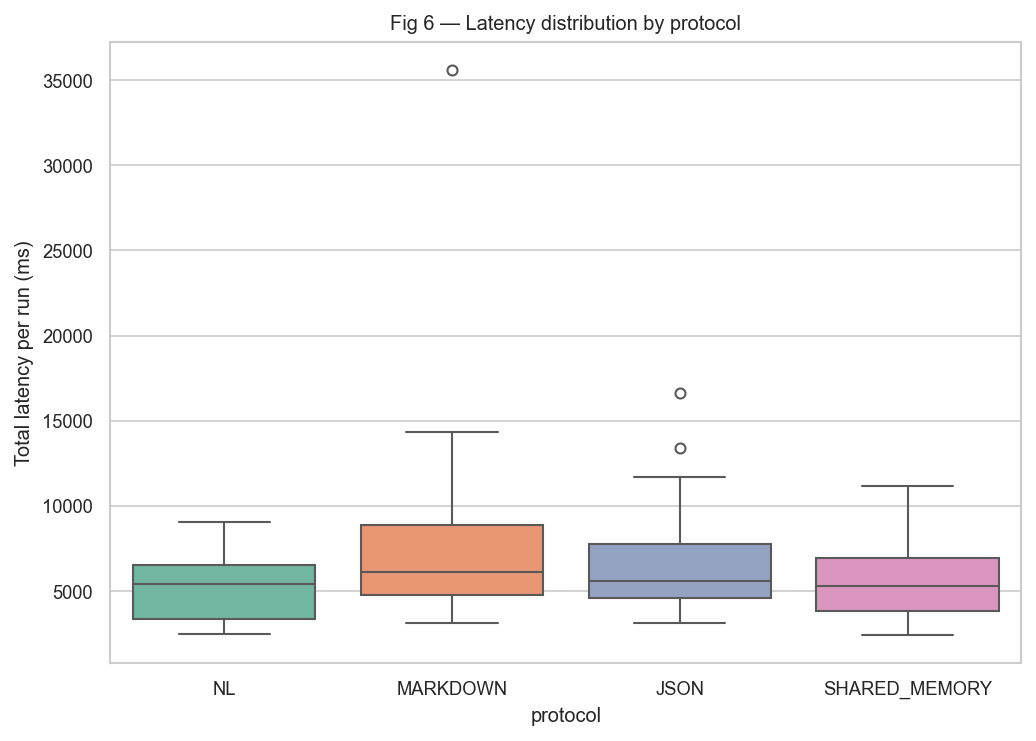
\includegraphics[width=\textwidth]{../figures/fig6_latency.png}
    \end{column}
    \begin{column}{0.39\textwidth}
      \textbf{Latency ANOVA}
      \begin{itemize}
        \item Protocol: $F=16.55$, $p<.001$, $\eta^2=.070$.
        \item Domain: $F=136.44$, $p<.001$, $\eta^2=.385$.
        \item Interaction: $F=6.38$, $p<.001$, $\eta^2=.054$.
      \end{itemize}

      \vspace{0.15cm}
      \textbf{Interpretation}
      \begin{itemize}
        \item Domain complexity dominates latency.
        \item Protocol still has a detectable operational effect.
        \item Token-efficient protocols also tend to reduce estimated API cost.
      \end{itemize}
    \end{column}
  \end{columns}
\end{frame}

\begin{frame}{Project Demo}
  \begin{columns}[T,onlytextwidth]
    \begin{column}{0.50\textwidth}
      \textbf{Streamlit workflow}
      \begin{enumerate}
        \item User enters a free-text task.
        \item LLM classifier predicts domain.
        \item App selects the empirically best protocol from \protocol{results\_summary.csv}.
        \item Planner, executor, and integrator run.
        \item Dashboard reports protocol, tokens, latency, cost, and final answer.
      \end{enumerate}
    \end{column}
    \begin{column}{0.46\textwidth}
      \begin{block}{Demo Contribution}
        The demo converts the offline benchmark into an actionable protocol-selection tool.
      \end{block}

      \vspace{0.2cm}
      \textbf{Implementation}
      \begin{itemize}
        \item Single-page Streamlit app in \protocol{app.py}.
        \item Auto-selection can be overridden manually.
        \item Raw message log exposes every inter-agent exchange for debugging.
      \end{itemize}
    \end{column}
  \end{columns}
\end{frame}

\begin{frame}{Limitations and Future Work}
  \begin{columns}[T,onlytextwidth]
    \begin{column}{0.48\textwidth}
      \textbf{Limitations}
      \begin{itemize}
        \item Sample size: 10 tasks per domain and 3 repetitions per cell.
        \item Single base model: all agents use \protocol{gpt-4o-mini}.
        \item Three-agent sequential chain only; no branching or debate.
        \item Completion interaction on quality is underpowered in the pooled test.
      \end{itemize}
    \end{column}
    \begin{column}{0.48\textwidth}
      \textbf{Next steps}
      \begin{itemize}
        \item Replicate with larger domain samples.
        \item Add XML, YAML, and hybrid protocols.
        \item Test heterogeneous agent models by role.
        \item Switch protocols dynamically based on confidence or token budget.
      \end{itemize}
    \end{column}
  \end{columns}
\end{frame}

\begin{frame}{Takeaways}
  \begin{enumerate}
    \item Communication protocol has a large efficiency effect: protocol explains $\eta^2=.262$ of token variance.
    \item Shared memory is consistently expensive, but improves completion on reading and news.
    \item Math is relatively insensitive to protocol quality; protocol choice there is mainly a cost decision.
    \item The project provides reusable artifacts: \protocol{pipeline.py}, 360-run results, figures, and a Streamlit demo.
  \end{enumerate}

  \vspace{0.35cm}
  \begin{block}{Final Recommendation}
    Do not choose a communication protocol globally. Choose it by domain and by whether the immediate priority is cost or completion quality.
  \end{block}
\end{frame}

\begin{frame}{Backup: Cell-Level Summary}
  \begin{table}
    \centering
    \scriptsize
    \begin{tabular}{llrrrr}
      \toprule
      Protocol & Domain & Tokens & Prompt & Completion & Score \\
      \midrule
      \protocol{NL} & Math & 988 & 665 & 323 & .833 \\
      \protocol{NL} & Reading & 819 & 717 & 102 & .426 \\
      \protocol{NL} & News & 995 & 680 & 315 & .275 \\
      \protocol{MARKDOWN} & Math & 1046 & 695 & 351 & .867 \\
      \protocol{MARKDOWN} & Reading & 995 & 794 & 201 & .347 \\
      \protocol{MARKDOWN} & News & 1433 & 860 & 574 & .271 \\
      \protocol{JSON} & Math & 847 & 600 & 247 & .733 \\
      \protocol{JSON} & Reading & 955 & 777 & 178 & .419 \\
      \protocol{JSON} & News & 1313 & 815 & 498 & .296 \\
      \protocol{SHARED\_MEMORY} & Math & 1204 & 931 & 273 & .833 \\
      \protocol{SHARED\_MEMORY} & Reading & 1192 & 1095 & 97 & .556 \\
      \protocol{SHARED\_MEMORY} & News & 1418 & 1052 & 366 & .346 \\
      \bottomrule
    \end{tabular}
  \end{table}

  \vspace{0.1cm}
  \centering
  \small Source: \protocol{results/results\_summary.csv}; each cell has $N=30$ runs.
\end{frame}

\end{document}
